\documentclass{article}
%% Useful packages
\usepackage[utf8]{inputenc}
\usepackage[a4paper,left=2cm,right=2cm,top=2cm,bottom=2cm]{geometry}
\usepackage{crop,graphicx,amsmath,array,color,amssymb,fancyhdr,lineno}
\usepackage{flushend,stfloats,amsthm,chngpage,times,,lipsum,lastpage} 
\usepackage{calc,listings,color,wrapfig,tabularx,longtable,enumitem}
\usepackage[style=numeric-comp,backend=biber,sorting=none]{biblatex}
\addbibresource{Refs.bib}
\usepackage{float}
\usepackage{enumitem}
\usepackage{xcolor}
\usepackage{hyperref}
\hypersetup{
    colorlinks=true,
    linkcolor=black,     
    urlcolor=blue,
    citecolor=purple
    }
\urlstyle{same}
%%%%%%%%%%%%   Header and Footer  %%%%%%%%%%%%%
\pagestyle{fancy}
\fancypagestyle{plain}{%
  \renewcommand{\headrulewidth}{0pt}%
  \fancyhf{}%
}

\title{%
  Project 1 \\
  \large Static analysis of a C code fragment using \textit{flawfinder}}
\author{Marco Ruvolo}

\begin{document}
\begin{titlepage}

\newcommand{\HRule}{\rule{\linewidth}{0.5mm}} % Defines a new command for the horizontal lines, change thickness here

%----------------------------------------------------------------------------------------
%	LOGO SECTION
%----------------------------------------------------------------------------------------
\center

\includegraphics[width=10cm]{Title/logo Sapienza (rgb).png}\\[1cm] % Include a department/university logo - this will require the graphicx package
 
%----------------------------------------------------------------------------------------

\center % Center everything on the page

%----------------------------------------------------------------------------------------
%	HEADING SECTIONS
%----------------------------------------------------------------------------------------

\textsc{\LARGE Sapienza University of Rome}\\[1.5cm] % Name of your university/college
\textsc{\Large Master's degree in Cybersecurity}\\[0.5cm] % Major heading such as course name
\textsc{\large Department of Computer Science}\\[0.5cm] % Minor heading such as course title

%----------------------------------------------------------------------------------------
%	TITLE SECTION
%----------------------------------------------------------------------------------------
\makeatletter
\HRule \\[0.4cm]
{ \huge \bfseries \@title}\\[0.4cm] % Title of your document
\HRule \\[1.5cm]
 
%----------------------------------------------------------------------------------------
%	AUTHOR SECTION
%----------------------------------------------------------------------------------------

\begin{minipage}{0.4\textwidth}
\begin{flushleft} \large
\emph{Author:}\\
\@author % Your name
\\[1.2em]
\emph{Matricola number:}\\
1883257 \\[1.2em]
\end{flushleft}
\end{minipage}
~
\begin{minipage}{0.4\textwidth}
\begin{flushright} \large
\emph{Professor:} \\
Daniele Friolo  \\[1.2em] % Supervisor's Name
\emph{Course:} \\
Security in Software Applications
\end{flushright}
\end{minipage}\\[2cm]
\makeatother

% If you don't want a supervisor, uncomment the two lines below and remove the section above
%\Large \emph{Author:}\\
%John \textsc{Smith}\\[3cm] % Your name

%----------------------------------------------------------------------------------------
%	DATE SECTION
%----------------------------------------------------------------------------------------
\vfill % Fill the rest of the page with whitespace
{\large \today}\\[2cm] % Date, change the \today to a set date if you want to be precise



\end{titlepage}

\sffamily

\fancyhf{}
\fancyhead[L]{}
\fancyhead[R]{}
\fancyfoot[R]{ \bf\thepage\ \rm }%

\newpage
\tableofcontents
\listoffigures
%\listoftables
\pagebreak

\section{Introduction to static analysis}

\subsection{Static analysis}
Static analysis is a set of techniques for verifying software without executing it (e.g., by examining the source code or the object code of a program).
Actually, there are different static analysis approaches and tools such as human analysis, type checkers, text scanners and many others.

Therefore, one of these static analysis tools will be described in the following subsection.

\subsection{A static analysis tool:  \textit{flawfinder}}
\textit{Flawfinder}\parencite{flawfinder} is a tool used to examine C/C++ source code and to report possible security vulnerabilities in the program.

On the one hand, this tool has various strenghts:
\begin{itemize}[itemsep=1.5pt]
    \item it works by using a built-in database of C/C++ functions with well-known problems (e.g., buffer overflows, \ldots) so you do not need to create this database by yourself;
    \item it carries out a list of potential security flaws (i.e., hits) sorted by risk and it may be able, in some cases, to determine that some construct are not dangerous at all, thus reducing false positives; 
    \item it can analyse software that you cannot build and it can even analyse files you cannot compile, in some cases;
    \item it gives finer information than simply running 'grep'\parencite{grep} Linux command on the source code (e.g., it knows to ignore comments and the insides of strings, it knows to examine parameters to estimate risk levels, \ldots).
\end{itemize}

On the other hand, \textit{flawfinder} has some weaknesses too:
\begin{itemize}[itemsep=1.5pt]
    \item it does not check on the data types of function arguments and it does not do control flow or data flow analysis at all (however, there exist other tools to analyse software more deeply);
    \item it does not understand the semantics of the code at all: it mainly does (simple) text pattern matching;
    \item it may report false positives (i.e., hits that are not actual security vulnerabilities);
    \item it may not necessarily find every security vulnerability in the program.
\end{itemize}

Summing up, \textit{flawfinder} is a simple tool that can be helpful in finding (and then removing) security vulnerabilities in C/C++ programs.
However, source code should nevertheless be inspected and evaluated to find possible vulnerabilities not reported by this tool.

\subsection{Project repository}
The project track carried out, the static analysis tool used, the different code fragment versions analysed, the images within this report and this latter itself, are collected in an online GitHub\parencite{github} repository.

For further information please visit the following link: \href{https://github.com/mrcruv/flawfinder_static_analysis}{https://github.com/mrcruv/flawfinder\_static\_analysis}.
\pagebreak

\section{A code fragment analysis}
\label{sec:analysis}

\subsection{Syntax error and warning fixing}
First of all (although \textit{flawfinder} can analyse files that cannot even be compiled), inspecting the original code fragment (see subsection \ref{app:A}), trying to compile it and fixing possible typos/syntax errors, is good practice before (actually, after as well) analysing software:

\begin{description}[itemsep=1.5pt]
    \item[warnings at lines 3, 4, 5, 6:] extra tokens at end of \#include directive $\xrightarrow{fix}$ the extra ';' tokens are removed at the end of each line;
    \item[warning at line 26] implicit declaration of function 'read'; did you mean 'fread'? $\xrightarrow{fix}$ the missing \#include directive for 'unistd.h'\parencite{unistd.h} is added;
    \item[error at line 27] 'buf' undeclared (first use in this function); did you mean 'buf2'? $\xrightarrow{fix}$ the suggested correction is applied;
    \item[warning at line 39:] implicit declaration of function 'error'; did you mean 'perror'? $\xrightarrow{fix}$ 'error' is reasonably replaced by 'fprintf'\parencite{fprintf} rather than by 'perror'\parencite{perror}, since 'errno'\parencite{errno} is not set;
    \item[error at line 54:] expected '\{' at end of input $\xrightarrow{fix}$ the missing '\{' at the end of line 47 is added;
    \item[warnings at line 55:] implicit declaration of function 'len' [-Wimplicit-function-declaration] $\xrightarrow{fix}$ 'len' is reasonably replaced by 'strlen'\parencite{strlen}; passing argument 1 of 'strlen' makes pointer from integer without a cast $\xrightarrow{fix}$ 'foo' is passed as the first argument of 'strlen' instead of '*foo'.
\end{description}
Please note that, with respect to the request to run \textit{flawfinder} before fixing typos, these fixes do not have a significant impact on the analysis performed.

\subsection{Security warning analysis}
Now, running \textit{flawfinder} on the "preprocessed" code fragment (see subsection \ref{app:B}) using the flag '-m 0' or '--minlevel=0', to set the minimum risk level to 0 (i.e., the minimum risk level can go from 0 - "no risk" - to 5 - "maximum risk" - and the default is 1) for inclusion in the hitlist (i.e., final results), carries out the analysis results.

The analysis summary shows that there are some possible security vulnerabilities in the code fragment, as can be seen from figure \ref{fig:analysis_summary}.

\begin{figure}[H]
    \centering
    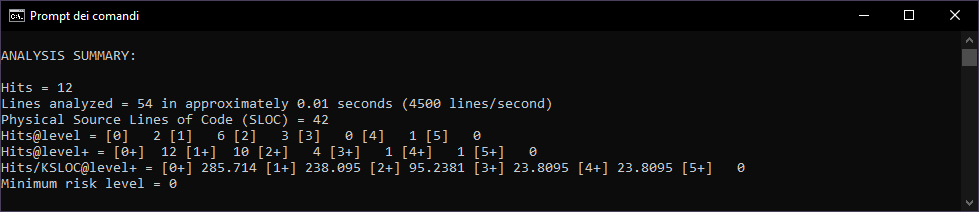
\includegraphics[width=0.9\textwidth]{Resources/analysis_summary.PNG}
    \caption{summary of the analysis of the code fragment (subsection \ref{app:B})}
    \label{fig:analysis_summary}
\end{figure}

In particular, the hits shown in the final results are twelve (mainly related to strings and buffer overflows), as can be seen from figure \ref{fig:final_results}:
\begin{description}[itemsep=1.5pt]
    \item[1) hit at line 52 (CWE-120\parencite{cwe-120}):] since the destination string 'buffer' is not large enough to receive the copy of the source string 'foo' the 'strcpy'\parencite{strcpy} invocation at line 52 will cause a buffer overflow, hence this hit is a vulnerability;
    \item[2) hit at line 10 (CWE-119!\parencite{cwe-119}/CWE-120):] since at line 13 'fgets'\parencite{fgets} is used to initialize 'buffer' and the second argument is set to the size in characters of 'buffer', 'buffer' will contain at most 1023 characters from 'stdin'\parencite{stdin} input channel (moreover, its 1024-th character will be the null byte), hence this hit is not a vulnerability (namely, 'buffer' is not improperly restricted);
    \item[3) hit at line 16 (CWE-119!/CWE-120):] since the destination string 'errormsg' is large enough to either receive the copy of the source string 'buffer' ('strncpy'\parencite{strncpy} at line 18) and to have the source string 'buffer' concatenated to itself ('strcat'\parencite{strcat} at line 19), and 'buffer' is null-terminated (by 'fgets' at line 13), this hit is not a vulnerability (namely, 'errormsg' is not improperly restricted) - moreover, 'errormsg' will be even null-terminated by 'strcat';
    \item[(4) hit at line 19 (CWE-120):] since 'errormsg' is large enough to store the result carried out by the invocation of 'strcat' at line 19, this hit is not a vulnerability;
    \item[(5) hit at line 18 (CWE-120):] since 'buffer' is null-terminated, after the 'strncpy' invocation at line 18, 'errormsg' will be null-terminated too, hence this hit is not a vulnerability;
    \item[6) hit at line 27 (CWE-120, CWE-20\parencite{cwe-20}):] since the third argument of 'read'\parencite{read} at line 27 is set to the size in bytes of 'len', this hit is not a vulnerability;
    \item[7) hit at line 29 (CWE-120, CWE-20):] since the third argument of 'read' at line 29 is set to the size (minus one) in characters (here, equal to the size in bytes minus one) of 'buf2', this hit is not a vulnerability;
    \item[8) hit at line 37 (CWE-120, CWE-20):] since the third argument of 'read' at line 37 is set to the size in bytes of 'buf3', this hit is not a vulnerability;
    \item[9) hit at line 45 (CWE-120, CWE-20):] since the third argument of 'read' at line 29 is set to the size in characters (here, equal to the size in bytes) of 'buf3', (yet 'buf3' will not be null-terminated in general: contrariwise, 'buf2' in 'func2' is explictly null-terminated at line 30), this hit is not a vulnerability (although all char buffers should be null-terminated);
    \item[10) hit at line 54 (CWE-126\parencite{cwe-126}):] since 'foo' is null-terminated by definition (even though the last character assigned to it is not explicitly the null byte, 'foo' is automatically null-terminated after being declared at line 49), this hit is not a vulnerability (namely, 'strlen' will not perform an over read);
    \item[11) hit at line 12 (CWE-134\parencite{cwe-134}):] since the format string passed as argument to 'printf'\parencite{printf} invocation at line 12 is constant, this hit is not a vulnerability (namely, no attacker can influence this format string);
    \item[12) hit at line 40 (CWE-134):] since the format string passed as argument to 'fprintf' invocation at line 40 is constant, this hit is not a vulnerability (namely, no attacker can influence this format string).
\end{description}

\begin{figure}[H]
    \centering
    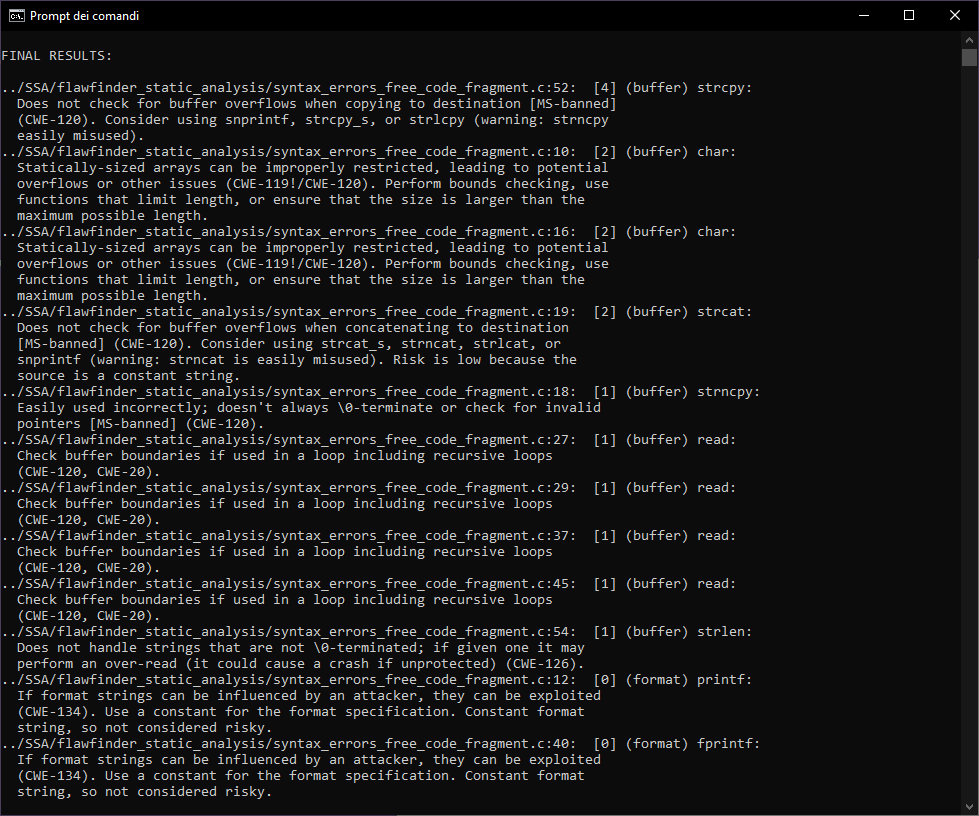
\includegraphics[width=0.9\textwidth]{Resources/final_results.PNG}
    \caption{final results of the analysis of the code fragment (subsection \ref{app:B})}
    \label{fig:final_results}
\end{figure}


\subsection{Other vulnerabilities and flaws}
Inspecting code again might help find other security vulnerabilities or simply weaknesses.

For instance, the following should be considered:
\begin{description}[itemsep=1.5pt]
    \item[return value checking:] with respect to each function invocation in the code, return values (if present) should be checked to determine whether a function (e.g., 'printf', 'fgets', 'malloc'\parencite{malloc}, 'read', \ldots) has been successfully executed or not;
    \item[exit in case of error:] when an error is detected it should be handled (e.g., terminating the code execution or trying again);
    \item[unsafe string library usage:] since some standard string library (i.e., 'string.h'\parencite{string.h}) functions (e.g., 'strcpy', \ldots) have been banned and have more robust or secure replacements (i.e., these functions are deprecated), a safe string library should be used instead (e.g., 'strsafe.h'\parencite{strsafe.h});
    \item[memory management:] with respect to memory allocation, 'calloc'\parencite{calloc} might be used rather than 'malloc' (e.g., to zero out memory in advance), furthermore allocated memory should be eventually released using 'free'\parencite{free};
    \item[explicit type casting:] when useful (e.g., 'calloc' return value, for code readability or disambiguation) or required (e.g., 'isalpha'\parencite{isalpha} checks argument to have the value of an
       unsigned char or EOF) explicit type conversion should be performed.
\end{description}
\pagebreak

\section{Vulnerability fixing}

At this point, a corrected version of the code fragment (see subsection \ref{app:C}) is produced by removing the security vulnerabilities found.

Here follows a summary of the vulnerability and flaw analysis performed in section \ref{sec:analysis}:
\begin{description}[itemsep=1.5pt]
    \item[1) vulnerability at line 52:] 'buffer' size is not large enough to receive the copy of 'foo';
    \item[2) flaws at multiple lines:] return values should be checked;
    \item[3) flaws at multiple lines:] errors should be handled;
    \item[4) flaws at multiple lines:] deprecated/unsafe string functions should be replaced by more robust or secure ones;
    \item[5) flaws at multiple lines:] memory management should be done properly;
    \item[6) flaws at multiple lines:] explicit type casting should be performed.
\end{description}

In practice, these latter are fixed in such a way:
\begin{description}[itemsep=1.5pt]
    \item[1), 2), 4):] 'strcpy' at line 52 is replaced by 'StringCbCopyA'\parencite{stringcbcopya} and a return value check is performed;
    \item[2):] a return value check is performed on 'printf' at line 12;
    \item[2):] a return value check is performed on 'fgets' at line 13;
    \item[2), 4):] 'strncpy' at line 18 is replaced by 'StringCbCopyA' and a return value check is performed;
    \item[2), 4):] 'strcat' at line 19 is replaced by 'StringCbCatA'\parencite{stringcbcata} and a return value check is performed;
    \item[2):] return value checks are performed on 'read' at lines 27, 29, 37, 45;
    \item[2), 5):] 'malloc' at lines 28, 44, 50 are replaced by 'calloc', return value checks are performed and memory is eventually deallocated using 'free';
    \item[2):] 'strlen' at line 54 (as argument of 'func3') is replaced by 'strnlen'\parencite{strnlen};
    \item[3):] in case of error (at lines 12, 13, 18, 19, 27, 28, 29, 37, 40, 44, 45, 50, 52), 'exit'\parencite{exit} is called ('EXIT\_FAILURE' is passed as argument);
    \item[6):] explicit type casting is performed ('isalpha' argument to 'unsigned char' at line 15 and 'calloc' return value to 'char *' at lines 28, 44).
\end{description}

Eventually, some minor corrections are made, for instance 'perror' is used to show messages on some standard errors (e.g., on 'read').

Please note that other message errors are not explicitly showed on 'stderr'\parencite{stdin} using 'fprintf', for the sake of brevity.
Moreover, neither a return value check is performed nor possible errors are handled on 'fprintf' at line 40 (this invocation works, in itself, as an error handler).

Now, running \textit{flawfinder} on the "fixed" code fragment using the flag '-m 0' or '--minlevel=0' (and ignoring the warnings that do not represent actual vulnerabilities by adding '// flawfinder: ignore' at the end of the involved lines in the code fragment) shows that all the vulnerabilities found have been removed, as can be seen from figure \ref{fig:final_results_and_analysis_summary_fixed}.
 \begin{figure}[H]
    \centering
    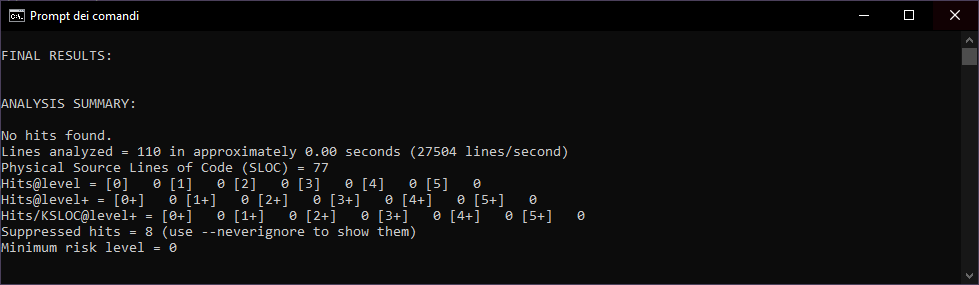
\includegraphics[width=0.9\textwidth]{Resources/final_results_and_analysis_summary_fixed.PNG}
    \caption{final results and summary of the analysis of the fixed code fragment (subsection \ref{app:C})}
    \label{fig:final_results_and_analysis_summary_fixed}
\end{figure}

\pagebreak

\printbibliography[heading=bibnumbered]
\pagebreak

\section{Appendixes}

\subsection{Appendix A}
\label{app:A}
\definecolor{dkgreen}{rgb}{0,0.6,0}
\definecolor{gray}{rgb}{0.5,0.5,0.5}
\definecolor{mauve}{rgb}{0.58,0,0.82}

\lstset{frame=tb,
  language=C,
  aboveskip=3mm,
  belowskip=3mm,
  showstringspaces=false,
  columns=flexible,
  basicstyle={\small\ttfamily},
  numbers=left,
  numberstyle=\tiny\color{gray},
  keywordstyle=\color{blue},
  commentstyle=\color{dkgreen},
  stringstyle=\color{mauve},
  breaklines=true,
  breakatwhitespace=true,
  tabsize=3
}
\begin{lstlisting}
// original code fragment:

#include <stdio.h>;
#include <ctype.h>;
#include <string.h>;
#include <stdlib.h>;

void func1() {	
    char buffer[1024];
    
    printf("Please enter your user id :");
    fgets(buffer, 1024, stdin);
     
    if (!isalpha(buffer[0])) {
        char errormsg[1044];
             
        strncpy(errormsg, buffer, 1024);
        strcat(errormsg, " is not  a valid ID");
 	}
}

void func2(int f2d) {
    char *buf2;
    size_t len;

    read(f2d, &len, sizeof(len));
    buf = malloc(len + 1);
    read(f2d, buf2, len);
    buf2[len] = '\0';
}

void func3(int f3d){
    char *buf3;
    int i, len;
         
    read(f3d, &len, sizeof(len));
         
    if (len > 8000) { 
        error("too large length"); 
        return; 
    }

    buf3 = malloc(len);
    read(f3d, buf3, len);    
}

void main()
    char *foo = "fooooooooooooooooooooooooooooooooooooooooooooooooooo";
    char *buffer = (char *)malloc(10 * sizeof(char));
    
    strcpy(buffer, foo);
    func1();
    func3(len(*foo));
}
\end{lstlisting}

\pagebreak

\subsection{Appendix B}
\label{app:B}
\definecolor{dkgreen}{rgb}{0,0.6,0}
\definecolor{gray}{rgb}{0.5,0.5,0.5}
\definecolor{mauve}{rgb}{0.58,0,0.82}

\lstset{frame=tb,
  language=C,
  aboveskip=3mm,
  belowskip=3mm,
  showstringspaces=false,
  columns=flexible,
  basicstyle={\small\ttfamily},
  numbers=left,
  numberstyle=\tiny\color{gray},
  keywordstyle=\color{blue},
  commentstyle=\color{dkgreen},
  stringstyle=\color{mauve},
  breaklines=true,
  breakatwhitespace=true,
  tabsize=3
}
\begin{lstlisting}
// syntax errors (and warnings) free code fragment:

#include <stdio.h>
#include <ctype.h>
#include <string.h>
#include <stdlib.h>
#include <unistd.h>

void func1() {	
    char buffer[1024];
    
    printf("Please enter your user id :");
    fgets(buffer, 1024, stdin);
     
    if (!isalpha(buffer[0])) {
        char errormsg[1044];
             
        strncpy(errormsg, buffer, 1024);
        strcat(errormsg, " is not  a valid ID");
 	}
}

void func2(int f2d) {
    char *buf2;
    size_t len;

    read(f2d, &len, sizeof(len));
    buf2 = malloc(len + 1);
    read(f2d, buf2, len);
    buf2[len] = '\0';
}

void func3(int f3d){
    char *buf3;
    int i, len;
         
    read(f3d, &len, sizeof(len));
         
    if (len > 8000) { 
        fprintf(stderr, "too large length"); 
        return; 
    }

    buf3 = malloc(len);
    read(f3d, buf3, len);    
}

void main() {
    char *foo = "fooooooooooooooooooooooooooooooooooooooooooooooooooo";
    char *buffer = (char *)malloc(10 * sizeof(char));
    
    strcpy(buffer, foo);
    func1();
    func3(strlen(foo));
}
\end{lstlisting}

\pagebreak

\subsection{Appendix C}
\label{app:C}
\definecolor{dkgreen}{rgb}{0,0.6,0}
\definecolor{gray}{rgb}{0.5,0.5,0.5}
\definecolor{mauve}{rgb}{0.58,0,0.82}

\lstset{frame=tb,
  language=C,
  aboveskip=3mm,
  belowskip=3mm,
  showstringspaces=false,
  columns=flexible,
  basicstyle={\small\ttfamily},
  numbers=left,
  numberstyle=\tiny\color{gray},
  keywordstyle=\color{blue},
  commentstyle=\color{dkgreen},
  stringstyle=\color{mauve},
  breaklines=true,
  breakatwhitespace=true,
  tabsize=3
}
\begin{lstlisting}
// fixed code fragment:

#include <stdio.h>
#include <ctype.h>
#include <string.h>
#include <stdlib.h>
#include <unistd.h>
#include <strsafe.h>

#define FUNC1_BUFFER_SIZE 1024
#define MAIN_BUFFER_SIZE 10

void func1() {	
    char buffer[FUNC1_BUFFER_SIZE]; // flawfinder: ignore
    int ret;
    HRESULT hr;
    
    ret = printf("Please enter your user id :"); // flawfinder: ignore
    
    if (ret < 0) exit(EXIT_FAILURE); // actually the condition to be verified would be 'ret < strnlen("Please enter your user id :", 29)'
    
    if (fgets(buffer, FUNC1_BUFFER_SIZE, stdin) == NULL) exit(EXIT_FAILURE);
    
    if (!isalpha((unsigned char)buffer[0])) {
        char errormsg[1044]; // flawfinder: ignore
        
        hr = StringCbCopyA(errormsg, FUNC1_BUFFER_SIZE, buffer);
        
        if (FAILED(hr)) exit(EXIT_FAILURE);
        
        hr = StringCbCatA(errormsg, 1044, " is not  a valid ID");
        
        if (FAILED(hr)) exit(EXIT_FAILURE);
 	}
}

void func2(int f2d) {
    char *buf2;
    size_t len;
    int ret;

    ret = read(f2d, &len, sizeof(len)); // flawfinder: ignore
    
    if (ret == -1) {
    	perror("error on first read (func2)");
		exit(EXIT_FAILURE); // errno is set
	}
	
    buf2 = (char *)calloc(len + 1, sizeof(char));
    
    if (buf2 == NULL) exit(EXIT_FAILURE);
    
    ret = read(f2d, buf2, len); // flawfinder: ignore
    
    if (ret == -1) {
    	perror("error on second read (func2)");
		exit(EXIT_FAILURE);
	}
	
    buf2[len] = '\0';
}

void func3(int f3d){
    char *buf3;
    int len, ret;
        
    ret = read(f3d, &len, sizeof(len)); // flawfinder: ignore
    
    if (ret == -1) {
    	perror("error on first read (func3)");
		exit(EXIT_FAILURE);
	}

    if (len > 8000) {
        fprintf(stderr, "error on too large length"); // flawfinder: ignore
        exit(EXIT_FAILURE);
    }

    buf3 = (char *)calloc(len, sizeof(char));
    
    if (buf3 == NULL) exit(EXIT_FAILURE);
    
    ret = read(f3d, buf3, len); // flawfinder: ignore
    
    free(buf3);
    buf3 = NULL;
    
    if (ret == -1) {
    	perror("error on second read (func3)");
		exit(EXIT_FAILURE);
	}
}

void main() {
    char *foo = "fooooooooooooooooooooooooooooooooooooooooooooooooooo";
    char *buffer = (char *)calloc(MAIN_BUFFER_SIZE, sizeof(char));
    HRESULT hr;
    
    if (buffer == NULL) exit(EXIT_FAILURE);
		
    hr = StringCbCopyA(buffer, MAIN_BUFFER_SIZE, foo);
	
    free(buffer);
    buffer = NULL;

    if (FAILED(hr) && hr != STRSAFE_E_INSUFFICIENT_BUFFER) exit(EXIT_FAILURE);
    
    func1();
    func3(strnlen(foo, 53));
    exit(EXIT_SUCCESS);
}
\end{lstlisting}

\pagebreak
\pagebreak

\end{document}
